\section{弱形式}
\label{sec:transp-weak}

三角形初值有折角，台阶初值有跳跃，这些初值都没有经典解的资格，可是特征线公式照样给出了合理的函数。怎样说它们“满足方程”？第~\ref{chap:pde-problems}章的办法是把导数转移到测试函数上。输运方程和连续性方程的导数位置不同，转移之后的结果也不同，所以要分别处理。

下面取$\Omega=\mathbb{R}^{d}$，设$\bm{v}$满足条件（V），测试函数$\psi\in C^{1}_{c}(\mathbb{R}^{d}\times[0,T))$，它在$t=T$附近为零，在$t=0$可以不为零。

\paragraph{两个弱形式}
设$u$是输运方程的经典解。乘以$\psi$，在$\mathbb{R}^{d}\times(0,T)$上积分。时间项对$t$分部积分，产生初值的边界项；空间项写成$\psi\bm{v}\cdot\nabla u$，对$\bm{x}$分部积分，导数要落到$\psi\bm{v}$上。

得到的关系里不再有$u$的导数，只有$\psi\bm{v}$的散度
\[
  \nabla\cdot(\psi\bm{v})=\bm{v}\cdot\nabla\psi+\psi\,\nabla\cdot\bm{v}.
\]

连续性方程的空间项本来就是散度，分部积分后导数只落在$\psi$上，$\bm{v}$不被求导。

\begin{definition}[输运方程与连续性方程的弱解]
\label{def:transp-weak}
设$u_0,\rho_0\in L^{1}_{\mathrm{loc}}(\mathbb{R}^{d})$，$f\in L^{1}_{\mathrm{loc}}(\mathbb{R}^{d}\times[0,T))$。称$u\in L^{1}_{\mathrm{loc}}(\mathbb{R}^{d}\times[0,T))$是输运方程的弱解，若对所有测试函数$\psi$，有
\begin{equation}
  \int_0^{T}\!\!\int u\bigl(\partial_t\psi+\nabla\cdot(\psi\bm{v})\bigr)\,\mathrm{d}\bm{x}\,\mathrm{d}t
  +\int u_0\,\psi(\cdot,0)\,\mathrm{d}\bm{x}
  +\int_0^{T}\!\!\int f\psi\,\mathrm{d}\bm{x}\,\mathrm{d}t=0.
  \label{eq:transp-weak-transport}
\end{equation}
称$\rho\in L^{1}_{\mathrm{loc}}(\mathbb{R}^{d}\times[0,T))$是连续性方程的弱解，若对所有测试函数$\psi$，有
\begin{equation}
  \int_0^{T}\!\!\int\rho\bigl(\partial_t\psi+\bm{v}\cdot\nabla\psi\bigr)\,\mathrm{d}\bm{x}\,\mathrm{d}t
  +\int\rho_0\,\psi(\cdot,0)\,\mathrm{d}\bm{x}
  +\int_0^{T}\!\!\int f\psi\,\mathrm{d}\bm{x}\,\mathrm{d}t=0.
  \label{eq:transp-weak-continuity}
\end{equation}
\end{definition}

两式都不含未知函数的导数，所以间断函数也可以代入。对比可以发现，式~\eqref{eq:transp-weak-transport}中出现了$\nabla\cdot\bm{v}$，要求速度场的散度是函数；式~\eqref{eq:transp-weak-continuity}只需要$\rho\bm{v}$局部可积，对$\bm{v}$的要求弱得多。

分部积分的步骤可逆，所以当$u$或$\rho$是$C^{1}$函数时，弱解就是经典解。下面用一个例子看看弱形式如何辨别间断的传播速度。

\begin{example}[台阶的传播速度]
\label{ex:transp-step}
取一维$v=1$，$f=0$，台阶初值$u_0=1$（$x<0$）、$u_0=0$（$x>0$）。考虑以速度$s>0$移动的台阶$u_s=1$（$x<st$）、$u_s=0$（$x>st$）。

把$u_s$代入式~\eqref{eq:transp-weak-transport}，记左端为$R(s)$，并令$I=\int_0^{T}\psi(st,t)\,\mathrm{d}t$。先算空间项，由微积分基本定理，
\[
  \int_0^{T}\!\!\int_{-\infty}^{st}\partial_x\psi\,\mathrm{d}x\,\mathrm{d}t=I.
\]

再算时间项。积分上限随时间移动，由含参积分的求导法则，
\[
  \frac{\mathrm{d}}{\mathrm{d}t}\int_{-\infty}^{st}\psi\,\mathrm{d}x=\int_{-\infty}^{st}\partial_t\psi\,\mathrm{d}x+s\psi(st,t).
\]
对$t$从$0$到$T$积分，
\[
  \int_0^{T}\!\!\int_{-\infty}^{st}\partial_t\psi\,\mathrm{d}x\,\mathrm{d}t
  =-\int_{-\infty}^{0}\psi(x,0)\,\mathrm{d}x-sI.
\]

两项相加，再加上初值项$\int_{-\infty}^{0}\psi(x,0)\,\mathrm{d}x$，初值积分抵消，
\[
  R(s)=(1-s)\,I.
\]
只要存在使$I\neq0$的测试函数，$R(s)=0$就等价于$s=1$。所以台阶的弱解只能以特征速度$1$移动。
\end{example}

图~\ref{fig:transp-weak-step}(a)的紫色等值线是一个测试函数，它跨在间断线的两侧。(b)用光滑的初值逼近台阶，光滑解$u_0^{\varepsilon}(x-t)$在$\varepsilon\to0$时收敛到台阶解，这也说明台阶解是光滑解的极限。(c)对一个具体的$\psi$计算了$R(s)$，绿点是数值积分的结果，只有$s=1$时为零。

\begin{BookInlineFigure}
  \centering
  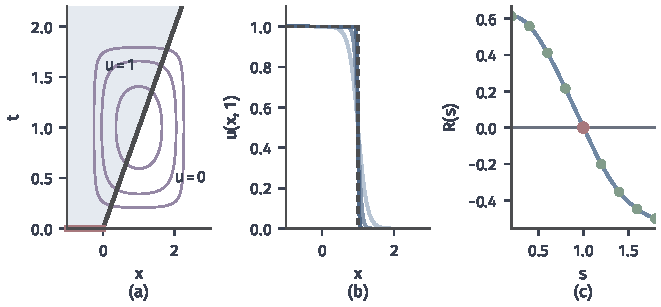
\includegraphics[width=112mm]{figures/06-differential-equations/02-partial-differential-equations/matplotlib/transp-weak-step/figure.pdf}
  \caption{台阶解的弱形式，$v=1$。(a)左侧浅蓝区域$u=1$，深灰粗线是间断线$x=t$，紫色曲线是测试函数$\psi$的等值线，红线是初值$1$的部分。(b)光滑化初值的解在$t=1$的剖面（蓝色由浅到深，过渡带越来越窄），虚线是台阶解。(c)$R(s)=(1-s)\int\psi(st,t)\,\mathrm{d}t$（蓝）与数值积分（绿），红点是$s=1$。}
  \label{fig:transp-weak-step}
\end{BookInlineFigure}

\paragraph{流构造就是弱解}
一般的情形下，第~\ref{sec:transp-flow}节的公式对粗糙的数据仍给出弱解，并且在$\bm{v}$足够正则时它是唯一的。

\begin{theorem}[流构造给出弱解]
\label{thm:transp-weak}
设$\bm{v}$满足条件（V）。
\begin{enumerate}
  \item 对$\rho_0\in L^{1}_{\mathrm{loc}}(\mathbb{R}^{d})$，函数
  \begin{equation}
    \rho(\bm{y},t)=\rho_0\bigl(\bm{\varphi}_{t,0}(\bm{y})\bigr)\,J_{t,0}(\bm{y})
    \label{eq:transp-weak-density}
  \end{equation}
  是连续性方程（$f=0$）的弱解，且是$L^{1}_{\mathrm{loc}}$中唯一的弱解。
  \item 对$u_0\in L^{1}_{\mathrm{loc}}(\mathbb{R}^{d})$，$u=u_0\circ\bm{\varphi}_{t,0}$是输运方程（$f=0$）的弱解。若$\nabla\cdot\bm{v}$还关于$\bm{x}$连续可微，这个弱解是$L^{1}_{\mathrm{loc}}$中唯一的。
\end{enumerate}
\end{theorem}

\begin{proof}
先证$\rho$是弱解。固定$\bm{x}$，由式~\eqref{eq:transp-flow}，沿轨迹有
\[
  \frac{\mathrm{d}}{\mathrm{d}t}\psi\bigl(\bm{\varphi}_{0,t}(\bm{x}),t\bigr)
  =\bigl(\partial_t\psi+\bm{v}\cdot\nabla\psi\bigr)\bigl(\bm{\varphi}_{0,t}(\bm{x}),t\bigr).
\]

在$[0,T]$上积分。$\psi$在$t=T$附近为零，于是
\[
  -\psi(\bm{x},0)=\int_0^{T}\bigl(\partial_t\psi+\bm{v}\cdot\nabla\psi\bigr)\bigl(\bm{\varphi}_{0,t}(\bm{x}),t\bigr)\,\mathrm{d}t.
\]

两边乘以$\rho_0(\bm{x})$，对$\bm{x}$积分并交换积分次序。式~\eqref{eq:transp-weak-density}的$\rho$满足式~\eqref{eq:transp-density}，换元$\bm{y}=\bm{\varphi}_{0,t}(\bm{x})$后，右端正是$\int_0^{T}\!\int\rho(\partial_t\psi+\bm{v}\cdot\nabla\psi)\,\mathrm{d}\bm{y}\,\mathrm{d}t$，这就是式~\eqref{eq:transp-weak-continuity}。

再证$u$是弱解。沿轨迹求导时多带一个因子$J_{0,t}$，由式~\eqref{eq:transp-liouville}，
\[
  \frac{\mathrm{d}}{\mathrm{d}t}\Bigl[\psi\bigl(\bm{\varphi}_{0,t}(\bm{x}),t\bigr)J_{0,t}(\bm{x})\Bigr]
  =\bigl(\partial_t\psi+\nabla\cdot(\psi\bm{v})\bigr)\bigl(\bm{\varphi}_{0,t}(\bm{x}),t\bigr)\,J_{0,t}(\bm{x}).
\]
对$t$积分，初值是$\psi(\bm{x},0)$。乘以$u_0(\bm{x})$，对$\bm{x}$积分，再把$\mathrm{d}\bm{x}$上的$J_{0,t}$用换元吸收，得到式~\eqref{eq:transp-weak-transport}。

接着证连续性方程的唯一性。设$\rho$是$\rho_0=0$的弱解，任取$h\in C^{1}_{c}(\mathbb{R}^{d}\times(0,T))$。定义
\[
  \psi(\bm{x},t)=-\int_t^{T}h\bigl(\bm{\varphi}_{t,r}(\bm{x}),r\bigr)\,\mathrm{d}r.
\]

由式~\eqref{eq:transp-flow-rules}，$\bm{\varphi}_{t,r}$是$\bm{\varphi}_{0,r}$与$\bm{\varphi}_{t,0}$的复合，关于$(\bm{x},t)$是$C^{1}$的，所以$\psi\in C^{1}$。$\psi$在$t=T$附近为零，$h$的支集紧，流映射连续，所以$\psi$的支集也紧，它是合法的测试函数。

任取一条轨迹$\bm{Y}(t)$，由定义，
\[
  \psi\bigl(\bm{Y}(t),t\bigr)=-\int_t^{T}h\bigl(\bm{Y}(r),r\bigr)\,\mathrm{d}r.
\]
对$t$求导，得到
\[
  \partial_t\psi+\bm{v}\cdot\nabla\psi=h.
\]
代入式~\eqref{eq:transp-weak-continuity}，得到
\[
  \int_0^{T}\!\!\int\rho h\,\mathrm{d}\bm{x}\,\mathrm{d}t=0.
\]
这对所有$h$成立，所以$\rho=0$几乎处处成立。

最后证输运方程的唯一性。令$c=\nabla\cdot\bm{v}$，取同样的$h$，定义
\[
  \psi(\bm{x},t)=-\int_t^{T}h\bigl(\bm{\varphi}_{t,r}(\bm{x}),r\bigr)\exp\Bigl(\int_t^{r}c\bigl(\bm{\varphi}_{t,\tau}(\bm{x}),\tau\bigr)\,\mathrm{d}\tau\Bigr)\mathrm{d}r.
\]

$c$关于$\bm{x}$是$C^{1}$的，所以$\psi\in C^{1}$，这就是额外假设的作用。沿轨迹用积分因子，得到$\partial_t\psi+\bm{v}\cdot\nabla\psi+c\psi=h$，即$\partial_t\psi+\nabla\cdot(\psi\bm{v})=h$。代入式~\eqref{eq:transp-weak-transport}，同样推出$u=0$。
\end{proof}

有源项时，解按式~\eqref{eq:transp-flow-solution}和式~\eqref{eq:transp-density-source}叠加，证明的计算相同，唯一性的结论也不变。

这个证明还揭示了两个方程之间的对偶关系。若$u$满足无源输运方程、$\rho$满足无源连续性方程，且二者足够光滑、衰减足够快，那么直接求导，用分部积分，可得
\[
  \frac{\mathrm{d}}{\mathrm{d}t}\int\rho u\,\mathrm{d}\bm{x}
  =\int\bigl(u\,\partial_t\rho+\rho\,\partial_tu\bigr)\,\mathrm{d}\bm{x}
  =\int\bigl(-u\nabla\cdot(\rho\bm{v})-\rho\bm{v}\cdot\nabla u\bigr)\,\mathrm{d}\bm{x}=0.
\]
也就是说，质量加权的标签总量不随时间变化。$h$与$\psi$的构造正是在利用这一点。

\paragraph{测度形式}
由于式~\eqref{eq:transp-weak-continuity}中不含$\bm{v}$的导数，也可以让$\rho_0$是测度。把积分$\int\rho_0\psi\,\mathrm{d}\bm{x}$换成$\int\psi\,\mathrm{d}\mu_0$，就可以描述集中在一点的质量。

取$\mu_0=\delta_{\bm{x}_0}$，式~\eqref{eq:transp-pushforward-measure}给出$\mu_t=\delta_{\bm{\varphi}_{0,t}(\bm{x}_0)}$，这个Dirac质量跟着粒子走。这是第~\ref{sec:transp-continuity}节密度搬运的极端情形，此时密度不再是函数，但质量守恒和推前关系仍然成立。

\paragraph{粗糙速度场}
以上结论都建立在条件（V）上。把$\bm{v}$换成粗糙的场，弱形式的写法没有变化，定理~\ref{thm:transp-weak}的结论却可能失效。

看图~\ref{fig:transp-rough-velocity}中的两个间断速度场。(a)$v=-\mathrm{sgn}(x)$：粒子从两侧撞向原点。$\rho_0=1$（$\lvert x\rvert<1$）时，$t<1$时的质量分布是
\begin{equation}
  \mu_t=\mathbf{1}_{\lvert x\rvert<1-t}\,\mathrm{d}x+2t\,\delta_0.
  \label{eq:transp-collision}
\end{equation}
质量在原点集中成Dirac，不再是函数。$\delta_0$处还需要规定$v$的取值，式~\eqref{eq:transp-collision}用的是$v(0)=0$，这个零测集上的取值现在影响结论。

(b)$v=\mathrm{sgn}(x)$：粒子从原点向两侧分开，$\lvert x\rvert<t$形成一块没有粒子来过的区域，浅红色部分。对输运方程来说，这里的值没有被初值决定。

对连续性方程，唯一性也会失败。看(c)：取$v=\mathrm{sgn}(x)$，初值$\rho_0=0$，定义
\begin{equation}
  \rho(x,t)=
  \begin{cases}
    t-x, & 0<x<t,\\
    -(t+x), & -t<x<0,\\
    0, & \text{其他}.
  \end{cases}
  \label{eq:transp-nonunique-density}
\end{equation}

\begin{BookInlineFigure}
  \centering
  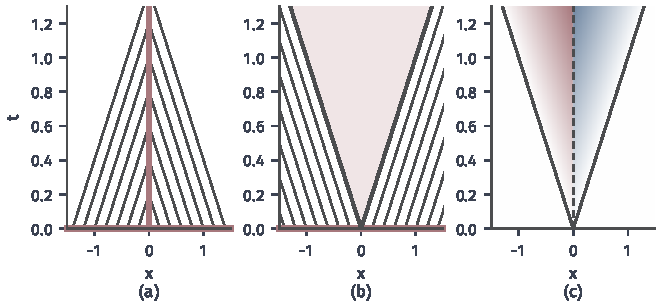
\includegraphics[width=112mm]{figures/06-differential-equations/02-partial-differential-equations/matplotlib/transp-rough-velocity/figure.pdf}
  \caption{间断速度场的三种问题，红线在(a)(b)中是初始线。(a)$v=-\mathrm{sgn}(x)$，特征线（深灰）撞向原点，红色粗线处积累质量。(b)$v=\mathrm{sgn}(x)$，浅红区域没有特征线到达。(c)$v=\mathrm{sgn}(x)$、$\rho_0=0$时的非零弱解~\eqref{eq:transp-nonunique-density}，红—白—蓝色阶的中点为$0$。}
  \label{fig:transp-rough-velocity}
\end{BookInlineFigure}

验证如下。在$x>0$的一侧，$v=1$，$\rho=t-x$满足$\partial_t\rho+\partial_x\rho=1-1=0$；$x<0$一侧，$v=-1$，$\rho=-(t+x)$满足$\partial_t\rho-\partial_x\rho=-1+1=0$。在分界线$x=0$上，右侧流量$\rho v=t\cdot1=t$，左侧流量$(-t)\cdot(-1)=t$，两侧相等，所以弱形式成立。

沿$x=\pm t$，$\rho$连续，没有问题。于是初值为零的问题有非零弱解，弱解在这里不唯一。式~\eqref{eq:transp-nonunique-density}的$\rho$有正有负，它在$x=0$两侧同时“产生”正、负质量。

这些例子都说明，弱形式并不会自动带来好的理论。超出Lipschitz范围的速度场需要专门的工具，结论依赖于$\nabla\bm{v}$的Sobolev型正则性和散度的有界性，这已超出本章的范围。本章的结论不能自动推广到任意粗糙的速度场。

\paragraph{有界区域上的弱形式}
有界区域的连续性方程也有相应的写法。要把$\Gamma_{-}$上的入流数据$g$放进去，测试函数应在$\Gamma_{+}$上为零。乘以$\psi$后分部积分，得到
\begin{equation}
  \int_0^{T}\!\!\int_{\Omega}\rho\bigl(\partial_t\psi+\bm{v}\cdot\nabla\psi\bigr)\,\mathrm{d}\bm{x}\,\mathrm{d}t
  +\int_{\Omega}\rho_0\psi(\cdot,0)\,\mathrm{d}\bm{x}
  +\int_0^{T}\!\!\int_{\Gamma_{-}}g\,\lvert\bm{v}\cdot\bm{n}\rvert\,\psi\,\mathrm{d}S\,\mathrm{d}t=0.
  \label{eq:transp-weak-boundary}
\end{equation}
边界项与式~\eqref{eq:transp-mass-rate}的入流项相对应，$\Gamma_{+}$上$\psi=0$让未知的出流值不进入方程。
